\documentclass[11pt, oneside]{article} 
\usepackage{geometry}
\geometry{letterpaper} 
\usepackage{graphicx}
	
\usepackage{amssymb}
\usepackage{amsmath}
\usepackage{parskip}
\usepackage{color}
\usepackage{hyperref}

\graphicspath{{/Users/telliott/Github/calculus_book/png/}}
% \begin{center} 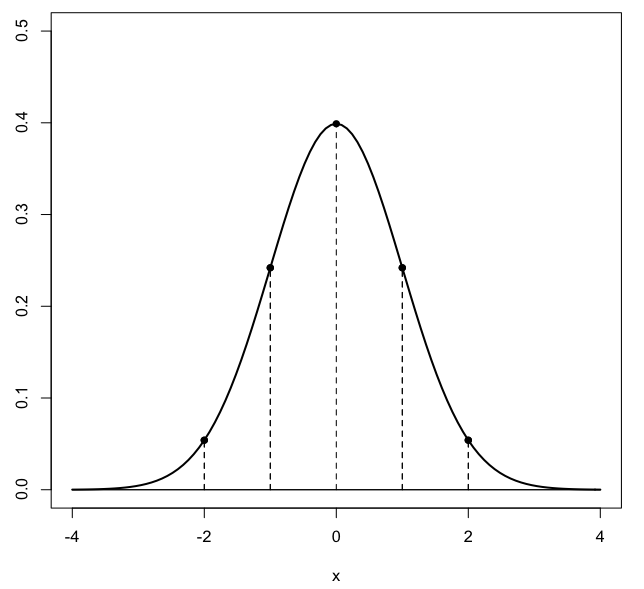
\includegraphics [scale=0.4] {gauss3.png} \end{center}

\title{Primes}
\date{}

\begin{document}
\maketitle
\Large

\subsection*{prime numbers}
As you know, positive integers larger than $1$ are of two types.  

$\circ$ \ a prime number $p$ has only two factors, $p$ and $1$

$\circ$ \ a composite number has at least one additional factor.  Either the number is a perfect square of a prime, or it has at least two additional factors.

The first few primes are:
\begin{verbatim}
2 3 5 7 11 13 17 19 23 29 ...
\end{verbatim}

\subsection*{The sieve of Eratosthenes}

Eratosthenes is famous in mathematics for his "sieve" which allows one to determine which numbers are prime in an economical fashion.  

We take note of him in talking about the circumference of the earth.  He was a contemporary of Archimedes and became the chief librarian at the Library of Alexandria when he was only about 35 years old.

The sieve operates by first writing down all the integers to some upper limit (here $120$).  To do things manually it is convenient to use rows with $10$ values, so there are $12$ rows in all here.  Most of the boxes have not yet been numbered (below, left).

Starting with the first prime number, $2$ (red), eliminate all the numbers divisible by $2$ (all the even numbers).  Here this has been done by coloring red all of the squares in the even numbered columns (all numbers ending in $2,4,6,8,0$).

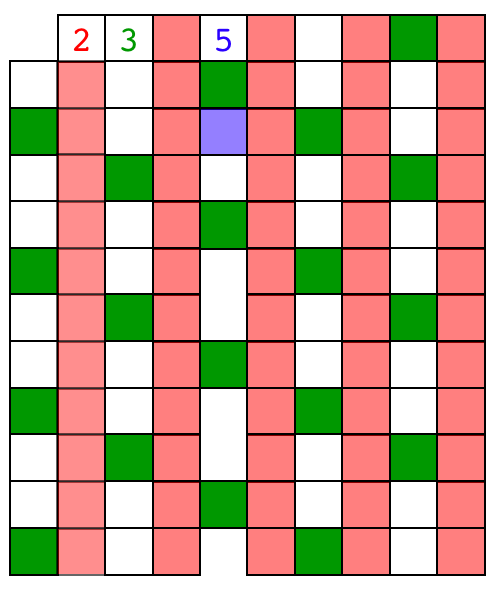
\includegraphics [scale=0.40] {sieve6.png}
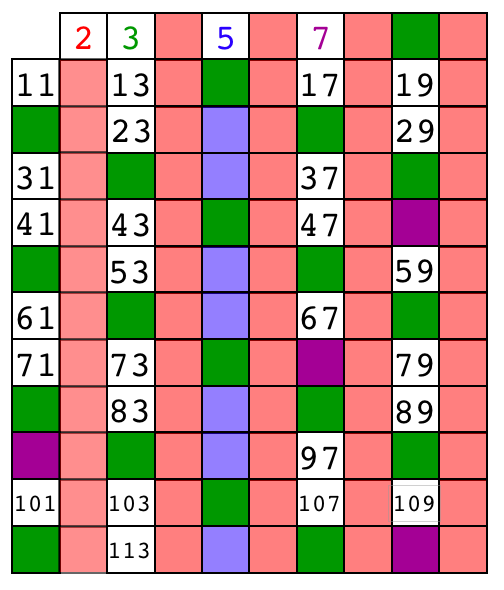
\includegraphics [scale=0.40] {sieve7.png}

Next, do the same thing with $3$ (green).  $6$ was already eliminated previously, but odd multiples of $3$ like $9$, $15$ and $21$ go away at this step.

The next larger number that still has a white square is $5$.  All the squares eliminated are white ones in the fifth row. The first value specifically eliminated at the $5$ step is $25$.  Continue with $7$, eliminating $49, 77, 91$ and $119$.

The sieve ends when the number for the beginning of the next round, the smallest number not yet eliminated, is larger than the square root of the upper limit (here $\sqrt{120}$).  So $7$ is used for the last round, because after that round the smallest remaining integer is $11$, but we terminate since $11^2 = 121 > 120$.

The graphic shows all the numbers which have yet to be eliminated after the round of $7$.   All of these numbers, $11$, $13$, $17$, and so on, as well as those used as divisors for each round of the sieve ($2, 3, 5, 7$), are prime numbers.

By testing for division by $2, 3, 5$ and $7$, we have found the first $30$ prime numbers.

From a performance standpoint, it is important that we do not need to carry out division.  All that is really needed is repeated addition.  Coding this algorithm in, say, Python is a good challenge.  A bigger challenge is to come up with a method to \emph{grow} the list of primes on demand.  This can be done by keeping track of the first value to be tested above the limit, for each prime in the current list.

\subsection*{infinite primes}

Euclid has a proof that the number of primes is infinite.

The proof is by contradiction:

Suppose the set of primes is finite, and that $p_1$, $p_2 \dots p_n$ are all of the primes.  Construct the following numbers:
\[ P = (p_1 \times p_2 \times \dots p_n)  \]
\[ Q = P + 1 \]
For a prime number $p$ to divide $Q$, it must divide the difference between $Q$ and $P$.  But that difference is $1$ and so can't be divided evenly by any prime.

Therefore, none of the known primes divides $Q$, and either

$\circ$ \  $Q$ is a prime not in the set of known primes

$\circ$ \ the set was originally incomplete.

In either case, the assumption that the set of primes is finite leads to a contradiction.

$\square$

Even for a relatively small number of primes, the second case may hold.  Consider
\[ (2 \cdot 3 \cdot 5 \cdot 7 \cdot 11 \cdot 13) + 1 = 30031 \]
$30031$ is not prime but is divided by two primes not in the list:  $59$ and $509$.

A different example is
\[ (2 \cdot 3 \cdot 7 \cdot 11) + 1 = 463 \]
$463$ is prime.

\subsection*{prime factorization}

We will prove that every integer has a unique prime factorization.  This is also called \emph{the fundamental theorem of arithmetic}.

\[ n = p_1 \cdot p_2 \dots p_n \]

In this list of prime factors, a factor may be repeated.  For example $12 = 2 \cdot 2 \cdot 3$.

First, we need a preliminary result called a lemma.  A lemma is like a mini-theorem, it needs to be proved first, and is then relied upon in the main part of the proof of a theorem.

Here, we assume Euclid's lemma is true.  For a proof, see

\url{https://en.wikipedia.org/wiki/Euclid%27s_lemma#Proof}

\subsection*{Euclid's lemma}

Every natural number $n > 1$, i.e. every positive integer greater than $1$, is either prime, or it is the product of two smaller natural numbers $a$ and $b$.

But the same is true of $a$ and $b$ in turn.

Therefore, every number that can be factored into $a$ and $b$ is the product of the prime factors of $a$ times the prime factors of $b$.  

The notation $m|n$ means $m$ divides $n$ (evenly).

Suppose a given prime $p$ divides $n = ab$, i.e. $p|n$.  Then either $p|a$ or  $p|b$ (or both).

$\square$

Below we will show a second proof of prime factorization that doesn't use Euclid's lemma, and then prime factorization can be used to prove the lemma.

\subsection*{Proof of prime factorization}

\subsection*{Existence}

The proof is by induction.

Assume the theorem is true for all numbers between $1$ and $n$.  

It is certainly true for say, $n \le 100$, because we can check each case.  Start with $n = 101$.

$\circ$ \ If $n$ is prime (as it is here) there is nothing to prove and we move to $n + 1$.  

$\circ$ \  $n$ is not prime, then there exist integers $a$ and $b$ (with $1 < a \le b < n$) such that $n = a \times b$.

$\circ$ \ By the induction hypothesis, since $a < n$ and $b < n$, $a$ has prime factors $p_1 p_2 \dots$ and $b$ has prime factors $q_1 q_2 \dots$ so
\[ n = ab = p_1 p_2 \dots q_1 q_2 \dots \]

This shows that there exists a prime factorization of $n$.

\subsection*{Uniqueness}

To show that the prime factorization is unique suppose that $n$ is the smallest integer for which there exist two different factorizations:
\[ n = p_1 p_2 \dots p_i \]
\[ = q_1 q_2 \dots q_j \]
    
Pick the first factor $p_1$.  Since $p_1$ divides $n = q_1 q_2 \dots$, by Euclid's lemma, it must divide some particular $q_j$.  Rearrange the $q$ so that particular $q_j$ is first.

But since $p_1$ divides $q_1$ and both are prime, it follows that $p_1 = q_1$. 

Now continue the same process with all the factors $p_i$.

wikipedia:

    This can be done for each of the $m$ $p_i$'s, showing that $m \le n$ and every $p_i$ is some $q_j$. Applying the same argument with the p and q reversed shows $n \le m$ (hence $m = n$) and every $q_j$ is a $p_i$.
    
$\square$
    
\subsection*{Second proof}

Hardy and Wright (\emph{Theory of Numbers}, sect. 2:11) have a different proof of prime factorization, which I find quite elegant and even delightful.

It is a proof by contradiction.

\begin{quote}Let us call numbers which can be factored into primes in more than one way, \emph{abnormal}, and let $n$ be the smallest abnormal number.\end{quote}

\subsection*{Different factorizations}

The same prime $P$ cannot appear in two different factorizations of $n$, for, if it did, $n/P$ would be abnormal and yet $n/P < n$, the smallest abnormal number.

Thus, we have that

\[  = p_1 p_2 \dots p_i = q_1 q_2 \dots q_j \]
    
where the $p$ and $q$ are primes, and no $p$ is a $q$ and no $q$ is a $p$.

If there exist abnormal numbers with two such factorizations, those factorizations must be completely different.

\subsection*{the contradiction, setup}

In this part, we establish that $p_1 \cdot q_1 < n$.

We may take $p_1$ to be the least $p$ and $q_1$ to be the least $q$.  

Since $n$ is composite, either $p_1$ is the only factor of $n$ (other than $1$ and $p$) and $p_1^2 = n$, or $p_1$ times the largest $p_j = n$, so $p_1 < p_j$, and $p_1^2 < n$.

A similar result holds for $q_1$.  

We also know that $p_1 \ne q_1$, so either $p_1^2 < n$ or $q_1^2 < n$ or both are true.

From all this, follows that $p_1 q_1 < n$. 

\subsection*{the contradiction} 

Let $N = n - p_1 q_1$.

We have $0 < N < n$ and also that $N$ is not abnormal.

Now $p_1 | n$ and given the above equality, it must be that $p_1 | N$.

A similar result is true for $q_1$, namely $q_1 | N$.  

Hence $p_1$ and $q_1$ both appear in the unique factorizations of both $N$ and $p_1 q_1$.

From this it follows that $p_1 q_1 | n$ and hence $q_1 = n/p_1$.  

But $n/p_1$ is less than $n$ and has the unique prime factorization $p_2 p_3 \dots$.

Since $q_1$ is not a $p$, this is impossible.  Hence there cannot be any abnormal numbers, and this is the fundamental theorem.

$\square$

\subsection*{Euclid's lemma, again}

Note:  since we just established the prime factorization theorem by the second proof, we can use it as a simple proof of Euclid's lemma.  

Suppose that $n=a \cdot b$.  If  $p | n$ then either $p | a$ or $p | b$ or both.

Proof:

Suppose to the contrary, $p | n$ but does not divide either $a$ or $b$.

Both $a$ and $b$ have a unique prime factorization and those factors multiplied together are the prime factors of $n$.  These factors do not include $p$, and yet the factorization is  unique.  This is a contradiction.

$p$ must divide either $a$ or $b$, or both.

$\square$

\end{document}